\chapter{人形机器人全身动作重定向}%20页


\section{引言}
人机交互(Human–Robot Interaction,HRI)是仿人机器人研究中的重要方向,而运动模仿则是实现自然、高效交互行为的核心手段之一。由于人体与机器人在运动学结构、关节自由度配置以及运动范围等方面存在显著差异,如何将人体动作合理映射到机器人平台上,仍然是运动模仿与动作重定向中的关键挑战。

现有的动作重定向方法通常可分为基于关节空间和基于笛卡尔空间的两类。前者侧重于保持人体与机器人在关节构型层面的相似性,但往往难以保证末端执行器在任务空间中的精确运动;后者则以末端轨迹跟踪为主要目标,但容易忽略整体肢体构型的一致性,从而导致机器人运动不自然。这种构型一致性与任务空间精度之间的权衡,限制了重定向结果在复杂交互场景中的适用性。

针对上述问题,本章在已有动作重定向研究的基础上,对传统重定向框架进行了改进,通过在关节空间构型约束与笛卡尔空间末端跟踪之间建立协调机制,实现了对人体上肢动作的有效映射。在保证机器人手臂整体构型与人体动作保持一致的同时,该方法能够显著提升末端执行器位置与姿态的跟踪精度,从而兼顾运动自然性与任务可执行性。实验结果表明,该重定向方法在不同动作类型与操作场景下均表现出良好的稳定性与适应性,为后续结合学习方法进行全身动作生成与控制奠定了基础。

近年来,利用人体运动数据对机器人进行示教与运动生成,已成为简化机器人运动编程与学习过程的一种重要途径 \cite{fu2024mobile, he2024learning, butepage2020imitating, kulic2016anthropomorphic}。通过观测和映射人类动作,机器人能够在无需显式建模复杂任务逻辑的情况下获得具有较强表现力和适应性的运动行为,这对于提升仿人机器人的自然性、自主性以及人机交互能力具有重要意义 \cite{chi2024universal, bahl2022human}。尽管该方向已取得一定进展 \cite{ishiguro2020bilateral, ramos2018humanoid},但在结构受限的真实机器人平台上实现稳定且精确的人体运动模仿,仍然面临诸多挑战 \cite{kim2009stable}。

从运动映射的角度来看,人体到机器人的动作模仿通常可抽象为一个\emph{动作重定向(motion retargeting)}问题,即在满足机器人自身运动学与动力学约束的前提下,将人体动作合理映射到机器人关节空间或任务空间中。由于人体与机器人在自由度数量、关节拓扑结构、运动范围以及力矩能力等方面存在显著差异,人体动作往往无法被机器人直接复现,这使得动作重定向成为运动模仿中的核心问题之一。

现有的动作重定向方法大致可以分为基于学习的方法和基于模型的方法。在动画与虚拟角色控制领域,强化学习被广泛用于从人体动作数据中学习复杂运动策略,并在多种任务中展现出良好的泛化能力与风格一致性 \cite{peng2018deepmimic, peng2021amp, won2020scalable, luo2023perpetual}。然而,将此类方法直接应用于真实仿人机器人仍然面临仿真到现实差距(sim-to-real gap)的问题,尤其是在关节力矩限制、硬件安全性以及高精度末端控制等方面存在明显挑战 \cite{bohez2022imitate, tang2024humanmimic}。

相比之下,基于模型的动作重定向方法由于其可解释性强、对物理约束处理明确,在真实机器人系统中仍被广泛采用。根据映射空间的不同,这类方法通常可进一步分为基于笛卡尔空间和基于关节空间的重定向策略。基于笛卡尔空间的方法通常以末端执行器位姿跟踪为主要目标,通过逆运动学或优化方法实现任务空间误差最小化 \cite{koenemann2014real, arduengo2021human}。这类方法在任务执行精度方面具有优势,但由于缺乏对整体肢体构型的约束,容易导致机器人运动不自然,且在存在避障或关节限制时可行性较差。相对而言,基于关节空间的方法更关注机器人与人体在构型层面的相似性,能够生成较为自然的运动,但往往难以保证末端执行器在任务空间中的精确跟踪,从而限制了其在精细操作任务中的应用。

因此,\textbf{如何在动作重定向过程中同时兼顾关节构型一致性与末端执行器的任务空间精度},成为当前类人机器人运动模仿研究中的一个关键问题。现有方法通常在这两者之间进行权衡,尚难以在统一框架下有效协调二者。

基于上述背景,本章在已有动作重定向研究的基础上,对传统的重定向流程进行了系统梳理与分析,并引入一种结合关节空间构型约束与笛卡尔空间任务优化的重定向建模思路。该思路以人体手臂运动为示教源,通过建立人体与机器人之间的几何对应关系,
在满足机器人关节空间约束的前提下,引入基于笛卡尔空间的优化机制,对末端执行器运动进行精确调节,从而在构型一致性与任务精度之间取得更为平衡的解。

需要强调的是,本章关注的重点在于\emph{动作重定向问题本身的建模方式与约束处理机制},其目的在于为后续章节中基于学习的全身动作生成与控制策略提供稳定、合理的低层动作映射基础。

\section{预备知识}

为后续人形机器人全身动作重定向与任务优先级控制模型的构建,本节对空间位姿描述与坐标变换方法,以及二次规划优化的基本理论进行简要回顾。这些内容构成后续全身运动学建模与优化求解的理论基础。



\subsection{空间位姿描述与坐标变换基础}

在人形机器人运动控制问题中,空间中任一点或刚体的状态通常由位置与姿态两部分组成。为统一描述空间几何关系,首先定义参考坐标系。设 $\{A\}$ 为参考坐标系,则空间点 $P$ 在坐标系 $\{A\}$ 下的位置向量表示为

\begin{equation}
	{}^{A}\mathbf{p} =
	\begin{bmatrix}
		p_x \\
		p_y \\
		p_z
	\end{bmatrix}.
\end{equation}

其中,上标 $A$ 表示该向量在坐标系 $\{A\}$ 下表达。图~\ref{fig:frameA} 给出了三维直角坐标系 $\{A\}$ 的示意图。

\begin{figure}[htbp]
	\centering
	\includegraphics[width=0.45\linewidth]{Figure/chapter2/frame_A.png}
	\caption{三维直角坐标系 $\{A\}$ 示意图}
	\label{fig:frameA}
\end{figure}

刚体姿态可通过附着于刚体的坐标系 $\{B\}$ 相对于参考系 $\{A\}$ 的关系描述。设 
$\{\hat{\mathbf{x}}_B,\hat{\mathbf{y}}_B,\hat{\mathbf{z}}_B\}$ 
为 $\{B\}$ 的三个单位基向量,则其在 $\{A\}$ 中的表达可构成旋转矩阵

\begin{equation}
	{}^{A}_{B}\mathbf{R} =
	\begin{bmatrix}
		{}^{A}\hat{\mathbf{x}}_B &
		{}^{A}\hat{\mathbf{y}}_B &
		{}^{A}\hat{\mathbf{z}}_B
	\end{bmatrix}.
\end{equation}

该旋转矩阵满足正交性条件

\begin{equation}
	{}^{A}_{B}\mathbf{R}^{T} \, {}^{A}_{B}\mathbf{R} = \mathbf{I}_3,
	\qquad
	{}^{A}_{B}\mathbf{R}^{-1} = {}^{B}_{A}\mathbf{R}.
\end{equation}

图~\ref{fig:frameAB} 给出了两个坐标系 $\{A\}$ 与 $\{B\}$ 的空间关系示意图。

\begin{figure}[htbp]
	\centering
	\includegraphics[width=0.75\linewidth]{Figure/chapter2/frame_A_B.png}
	\caption{坐标系 $\{A\}$ 与 $\{B\}$ 的空间关系示意图}
	\label{fig:frameAB}
\end{figure}

若两个坐标系原点重合,仅存在旋转关系,则任意向量在两个坐标系中的表达满足
${}^{A}\mathbf{p} = {}^{A}_{B}\mathbf{R}\,{}^{B}\mathbf{p}$。若两坐标系姿态相同,仅存在平移关系,则有
${}^{A}\mathbf{p} = {}^{B}\mathbf{p} + {}^{A}\mathbf{p}_{B\mathrm{ORG}}$。其中 ${}^{A}\mathbf{p}_{B\mathrm{ORG}}$ 表示坐标系 $\{B\}$ 原点在 $\{A\}$ 下的位置。

综合平移与旋转,可构造齐次变换矩阵

\begin{equation}
	{}^{A}_{B}\mathbf{T} =
	\begin{bmatrix}
		{}^{A}_{B}\mathbf{R} & {}^{A}\mathbf{p}_{B\mathrm{ORG}} \\
		\mathbf{0}_{1\times 3} & 1
	\end{bmatrix}
	\in SE(3),
\end{equation}

则空间点在不同坐标系之间的映射关系可统一表示为

\begin{equation}
	\begin{bmatrix}
		{}^{A}\mathbf{p} \\
		1
	\end{bmatrix}
	=
	{}^{A}_{B}\mathbf{T}
	\begin{bmatrix}
		{}^{B}\mathbf{p} \\
		1
	\end{bmatrix}.
\end{equation}

上述空间位姿表示与坐标变换关系构成了人形机器人几何建模的基础框架,为后续全身运动学推导以及人体动作到机器人结构之间的重定向映射提供了统一的数学描述形式。



\subsection{二次规划与约束优化基础}
二次规划(Quadratic Programming, QP)的一般形式为
\begin{equation}
	\begin{aligned}
		\min_{\mathbf{x}} \quad &
		\frac{1}{2}\mathbf{x}^T \mathbf{G}\mathbf{x}
		+
		\mathbf{h}^T \mathbf{x} \\
		\text{s.t.} \quad &
		\mathbf{A}\mathbf{x} = \mathbf{b}, \\
		&
		\mathbf{C}\mathbf{x} \le \mathbf{d},
	\end{aligned}
	\label{eq:qp_general}
\end{equation}
其中 $\mathbf{G} \succeq 0$ 为半正定矩阵,$\mathbf{A}\mathbf{x} = \mathbf{b}$ 和 $\mathbf{C}\mathbf{x} \le \mathbf{d}$ 分别表示等式与不等式约束。

当仅存在等式约束时,可构造 Lagrange 函数
\begin{equation}
	\mathcal{L}(\mathbf{x},\boldsymbol{\lambda})
	=
	\frac{1}{2}\mathbf{x}^T \mathbf{G}\mathbf{x}
	+
	\mathbf{h}^T \mathbf{x}
	+
	\boldsymbol{\lambda}^T(\mathbf{A}\mathbf{x}-\mathbf{b}),
\end{equation}
对 $\mathbf{x}$ 与 $\boldsymbol{\lambda}$ 求偏导并令其为零,可得到一阶最优性条件,整理后得到 KKT 方程组
\begin{equation}
	\begin{bmatrix}
		\mathbf{G} & \mathbf{A}^T \\
		\mathbf{A} & \mathbf{0}
	\end{bmatrix}
	\begin{bmatrix}
		\mathbf{x} \\
		\boldsymbol{\lambda}
	\end{bmatrix}
	=
	\begin{bmatrix}
		-\mathbf{h} \\
		\mathbf{b}
	\end{bmatrix},
\end{equation}
通过求解该线性方程组即可获得二次规划问题的最优解。

另一方面,在人形机器人运动学中,设广义关节变量为 $\mathbf{q} \in \mathbb{R}^n$,任务空间变量记为 $\mathbf{x}$,则末端或任务点的位姿满足
\begin{equation}
	\mathbf{x} = f(\mathbf{q}),
\end{equation}
其微分形式为
\begin{equation}
	\dot{\mathbf{x}} = \mathbf{J}(\mathbf{q}) \dot{\mathbf{q}},
	\label{eq:task_velocity_mapping}
\end{equation}
其中 $\mathbf{J}(\mathbf{q})$ 为雅可比矩阵。

给定期望的任务空间速度 $\dot{\mathbf{x}}_d$,可以构造任务空间速度误差
\begin{equation}
	\mathbf{e}_v = \mathbf{J}(\mathbf{q}) \dot{\mathbf{q}} - \dot{\mathbf{x}}_d,
\end{equation}
并以其加权二范数作为代价函数
\begin{equation}
	\min_{\dot{\mathbf{q}}} \;
	\frac{1}{2} \mathbf{e}_v^T \mathbf{W} \mathbf{e}_v
	=
	\frac{1}{2}
	\big(
	\mathbf{J}(\mathbf{q}) \dot{\mathbf{q}} - \dot{\mathbf{x}}_d
	\big)^T
	\mathbf{W}
	\big(
	\mathbf{J}(\mathbf{q}) \dot{\mathbf{q}} - \dot{\mathbf{x}}_d
	\big),
	\label{eq:quadratic_cost_from_jacobian}
\end{equation}
其中 $\mathbf{W} \succeq 0$ 为任务空间加权矩阵。展开式\eqref{eq:quadratic_cost_from_jacobian} 可得
\begin{equation}
	\frac{1}{2} \dot{\mathbf{q}}^T \big( \mathbf{J}^T \mathbf{W} \mathbf{J} \big) \dot{\mathbf{q}}
	-
	\big( \mathbf{J}^T \mathbf{W} \dot{\mathbf{x}}_d \big)^T \dot{\mathbf{q}}
	+
	\text{const},
\end{equation}
从而可以识别出
\begin{equation}
	\mathbf{x} \equiv \dot{\mathbf{q}}, \quad
	\mathbf{G} = \mathbf{J}^T \mathbf{W} \mathbf{J}, \quad
	\mathbf{h} = - \mathbf{J}^T \mathbf{W} \dot{\mathbf{x}}_d,
\end{equation}

即由机器人雅可比映射自然得到二次规划中的二次型代价形式。进一步结合关节速度限制、末端约束等线性约束,即可将全身运动学问题统一表示为式\eqref{eq:qp_general} 所示的标准 QP 形式,为后续的人形机器人动作重定向提供统一的优化求解框架。




\section{方法}
\subsection{动作模仿系统设计}
图~\ref{fig:System_Block_Diagram} 展示了本文所构建的全身动作模仿系统整体框架。系统主要由视觉采集系统、上位处理器、下位处理器以及机械运动系统四个部分组成,各模块协同工作以实现人形机器人全身动作模仿。

\begin{figure}[htbp]
	\centering
	\includegraphics[width=0.9\linewidth]{Figure/chapter2/system_frame.png}
	\caption{全身动作模仿系统整体框架}
	\label{fig:System_Block_Diagram}
\end{figure}

视觉采集系统采用标准的 RGB-D 摄像设备,本文实验中使用 Intel RealSense D435 深度相机。摄像头安装于被试者正前方,距地面约 1.5 m,用于实时获取人体运动图像及对应的深度信息。采集到的数据通过 USB 接口传输至上位处理器进行处理。

上位处理器为一台 PC,负责完成人体姿态信息的提取与预处理。具体而言,上位处理器对输入的 RGB 图像进行人体姿态估计,提取人体全身关键点的二维信息,并进一步结合深度数据恢复三维关键点位置。为降低传感噪声对后续动作重定向的影响,本文对三维关键点序列引入卡尔曼滤波进行平滑处理。处理后的关键点数据通过 ROS 通信机制发送至下位处理器。

为清晰描述人体与机器人之间的映射关系,
图~\ref{fig:human_robot_compare} 给出了人体关键点结构与机器人本体结构的对比示意图。
图~\ref{fig:human_keypoints_sub} 为人体关键点定义,
图~\ref{fig:robot_structure_sub} 为机器人本体结构及关节坐标系定义。

\begin{figure}[htbp]
	\centering
	\begin{subfigure}[b]{0.32\textwidth}
		\centering
		\includegraphics[width=\linewidth]{Figure/chapter2/human_body.png}
		\caption{人体关键点定义}
		\label{fig:human_keypoints_sub}
	\end{subfigure}
	\hfill
	\begin{subfigure}[b]{0.52\textwidth}
		\centering
		\includegraphics[width=\linewidth]{Figure/chapter2/M04_body.png}
		\caption{人形机器人本体结构与关节旋转}
		\label{fig:robot_structure_sub}
	\end{subfigure}
	\caption{人体关键点与机器人本体结构对比示意图}
	\label{fig:human_robot_compare}
\end{figure}

人体侧关键点包括肩关节($S$)、肘关节($E$)、腕关节($W$)、髋关节($H$)、膝关节($K$)、踝关节($A$)以及躯干参考点($P$、$O$)等。通过人体姿态估计算法可获取上述关键点在相机坐标系下的三维空间位置坐标,从而构建人体全身骨架的几何拓扑结构。机器人侧则建立与人体结构相对应的串联关节连杆模型,并在各关节处定义局部连杆坐标系 $\{X,Y,Z\}$。各关节旋转采用右手坐标系约定,并按照 Roll–Pitch–Yaw 顺序定义转动自由度。该统一的坐标描述方式为人体—机器人之间的几何映射与运动学重定向提供了理论基础。

下位处理器用于执行动作重定向计算与机器人控制指令生成。在接收到人体三维关键点数据后,系统首先基于人体几何模型计算对应的人体关节角度,该关节角度作为机器人动作重定向问题的初始参考。随后,通过迭代优化求解满足机器人关节物理约束并同时逼近人体末端运动目标的关节角解。最终得到的目标关节角通过 CAN 总线发送至机械运动系统,用于驱动机器人执行相应的全身动作。

机械运动系统由机器人双臂、双腿、电机及其驱动模块构成。本文所使用的仿人机器人平台为自主研发系统。上肢每条机械臂具有六个自由度,包括肩关节三自由度(屈伸、外展内收、旋内外)、肘关节屈伸、前臂旋前旋后以及腕关节屈伸;下肢包括髋关节三自由度、膝关节屈伸以及踝关节俯仰。该结构能够满足机器人在三维空间内完成复杂全身动作的运动学需求,为人体动作的有效重定向提供了硬件基础。


\section{改进重定向}

\subsection{人体肩关节几何建模}
由于肩关节和肘关节主要影响手臂的运动,而手腕主要影响手的运动,本研究重点对肩关节和肘关节进行几何建模。为清楚说明肩关节和肘关节的建模方法,下面以左臂的建模过程进行说明。

如图 \ref{fig:Modeling_of_shoulder} 所示,点 $S$ 表示左臂的肩关节,点 $E$ 表示左臂的肘关节,点 $M$ 则位于 Y 轴上,距离为 $a$ 的一点。
\begin{figure}[h]
	\centering
	\includegraphics[width=0.4\textwidth]{Figure/chapter2/Fig3.png}
	\caption{左手肩关节建模。}
	\label{fig:Modeling_of_shoulder}
\end{figure}


根据上述定义,可以证明 $|\bm{SM}| = a$。通过姿态估计,可以获得各关键点在相机坐标系下的坐标,分别为 $S(x_0, y_0, z_0)$、$E(x_1, y_1, z_1)$ 以及 $M(x_0, y_0 - a, z_0)$。以点 $S$ 为原点建立肩关节局部坐标系后,各点在该坐标系下的坐标可表示为 $S(0, 0, 0)$、$E(x_1 - x_0,\, y_1 - y_0,\, z_1 - z_0)$ 以及 $M(0,\, -a,\, 0)$。

点 $E$ 在平面 $(ZSM)$ 上的正交投影记为点 $F$,其坐标为 $F(0,\, y_0 - y_1,\, z_1 - z_0)$。向量 $\bm{SE}$ 在平面 $(ZSM)$ 上的投影与 $Y$ 轴负方向之间的夹角定义为 $\theta_{SP}$,即 $\angle FSM = \theta_{SP}$,其中 $\theta_{SP}$ 表示肩关节的屈伸角;向量 $\bm{SE}$ 与其在平面 $(ZSM)$ 上投影之间的夹角定义为 $\theta_2$,即 $\angle FSE = \theta_{SR}$,其中 $\theta_{SR}$ 表示肩关节的外展–内收角。

在上述几何关系下,可在三角形 $\triangle FSM$ 中求解角度 $\theta_{SP}$,根据余弦定理有
\begin{equation}
\theta_{SP}
= \arccos\!\left(
\frac{|\bm{SF}|^{2} + |\bm{SM}|^{2} - |\bm{FM}|^{2}}
{2\,|\bm{SF}|\,|\bm{SM}|}
\right)
= \arccos\!\left(
\frac{y_0 - y_1}{|\bm{SF}|}
\right),
\label{eq:theta1}
\end{equation}

其中角度 $\theta_{SP}$ 的符号可由 $z_1 - z_0$ 的符号确定:当 $z_1 - z_0 > 0$ 时,表示手臂向前摆动;当 $z_1 - z_0 < 0$ 时,表示手臂向后摆动。同理,在三角形 $\triangle FSE$ 中可求解肩关节外展–内收角 $\theta_{SR}$,其表达式为

\begin{equation}
\theta_{SR}
= \arccos\!\left(
\frac{|\bm{SF}|^{2} + |\bm{SE}|^{2} - |\bm{FE}|^{2}}
{2\,|\bm{SF}|\,|\bm{SE}|}
\right).
\label{eq:theta2}
\end{equation}



\subsection{人体肘关节几何建模}
如图~\ref{fig:Modeling of elbow}(\textbf{a}) 所示,$W$ 表示手腕的实际位置,$W'$ 表示手腕的假定初始位置(此时 $\theta_{SY} = 0$)。角度 $\theta_{SY}$ 定义为从肘部指向手腕的向量 $\bm{EW}$ 与其初始位置向量 $\bm{EW'}$ 之间的夹角;角度 $\theta_{E}$ 定义为向量 $\bm{EW}$ 与向量 $\bm{SE}$ 的延长线之间的夹角。


\begin{figure}[H]
	\centering
	%\isPreprints{}{% This command is only used for ``preprints''.
		\begin{adjustwidth}{0cm}{0cm}
			\subfloat[\centering]{\includegraphics[width=7.5cm]{Figure/chapter2/Fig4.png}}
			\label{fig:arm joint angles are non zero}
			\hfill
			\subfloat[\centering]{\includegraphics[width=5.4cm]{Figure/chapter2/Fig5.png}}
			\label{fig:arm joint angles are zero}
			
		\end{adjustwidth}
  \caption{肘关节建模。(\textbf{a})当手臂关节角不为零时的肘关节坐标系,其中 $\theta_{SY}$ 表示肩关节外-内旋角,$\theta_{E}$ 表示肘关节屈伸角的补角。(\textbf{b})当手臂所有关节角均为零时的肘关节坐标系。}
		\label{fig:Modeling of elbow}
	\end{figure} 

当手腕位于位置 $W'$ 时,肘关节的局部坐标系记为 $E X_{1} Y_{1} Z_{1}$。假设手臂的初始状态为 $\theta_{SP}$、$\theta_{SR}$、$\theta_{SY}$ 和 $\theta_{E}$ 均为零,则此时肘关节坐标系的定义如图~\ref{fig:Modeling of elbow}(\textbf{b}) 所示。


通过姿态估计,可以获得点 $S$、$E$ 和 $W$ 在相机坐标系下的绝对坐标,分别为 $S(x_{0}, y_{0}, z_{0})$、$E(x_{1}, y_{1}, z_{1})$ 和 $W(x_{2}, y_{2}, z_{2})$。在以肩关节为原点建立的相对坐标系下,手腕点 $W$ 的坐标可表示为 $W(x_{2}-x_{0},\, y_{2}-y_{0},\, z_{2}-z_{0})$。

如图 \ref{fig:Modeling of elbow}(\textbf{a}) 所示,在以肩关节为原点建立的相对坐标系中,肩关节外旋角 $\theta_{E}$ 可通过向量 $\bm{SE}$ 与向量 $\bm{EW}$ 的点积计算得到。


\begin{eqnarray}
\theta_{E} = \arccos\left[\frac{\bm{SE}\cdot\bm{EW}}{|\bm{SE}||\bm{EW}|}\right]
\end{eqnarray}

人体肘关节的活动范围为 $\pi - \theta_{E}$,其中向量 $\bm{EW}$ 的坐标为 $(x_{1} - x_{2},\, y_{1} - y_{2},\, z_{2} - z_{1})$。

为求解 $\theta_{SY}$,已知实际手腕位置 $W$,首先需要计算向量 $\bm{HW}$。如图 \ref{fig:Modeling of elbow}(\textbf{a}) 所示,$Y_1$ 轴定义为始终指向肩关节到肘关节的连线,即沿向量 $\bm{SE}$ 的方向。由于 $\theta_{E}$ 已确定,无论 $\theta_{SY}$ 如何变化,向量 $\bm{EW}$、$\bm{EW'}$ 与 $\bm{EH}$(即 $Y_1$ 轴)之间的夹角均保持为 $\theta_{E}$,换言之,连接肘关节与手腕的线 $\bm{EW'}$ 围绕 $Y_1$ 轴旋转形成向量 $\bm{EW}$。


\begin{gather}
|\bm{EW'}|= |\bm{EW}| \\
|\bm{EH}|= |\bm{EW'}|*cos\theta_{E} \\
\bm{EH} =|\bm{EH}|\ast\frac{\bm{SE}}{|\bm{SE}|}
\end{gather}

因此,通过 $\bm{HW} = \bm{EW} - \bm{EH}$ 可以得到向量 $\bm{HW}$。需要注意的是,虽然肩关节坐标系在手臂运动过程中保持固定,但肘关节坐标系会随姿态变化而改变方向,如图 \ref{fig: Rotational schematic of the shoulder coordinate system} 所示。在手臂运动过程中,肘关节坐标系会旋转到新的状态。在图 \ref{fig: Rotational schematic of the shoulder coordinate system} 中,$Z_1$ 轴的方向会随着 $\theta_{SP}$ 的值而变化,$Z_1'$ 轴表示 $Z_1$ 轴从肘关节平移到肩关节的位置。沿 $Z_1'$ 轴的方向向量记为 $\bm{p}$,且满足 $\bm{p} \perp \bm{m}$ 且 $|\bm{p}| = 1$,因此 $\bm{p} = (0, \sin\theta_1, -\cos\theta_1)$。如图所示,$\bm{p}$ 表示当手腕达到位置 $W'$ 时,肘关节处 $Z_1$ 轴的方向。已知向量 $\bm{HW}$ 以及与 $\bm{HW'}$ 平行的方向向量 $\bm{p}$,即可求得 $\theta_{SY}$。


\begin{figure}[H]
\centering
%\isPreprints{}{% This command is only used for ``preprints''.
	\begin{adjustwidth}{0cm}{0cm}
		\subfloat[\centering]{\includegraphics[width=5cm]{Figure/chapter2/Fig6_a.png}}
		\label{fig: Shoulder motion as an acute angle}
		\hfill
		\subfloat[\centering]{\includegraphics[width=5cm]{Figure/chapter2/Fig6_b.png}}
		\label{fig: Shoulder motion as an obtuse angle}
		
	\end{adjustwidth}
\caption{手臂运动过程中肩关节坐标系的旋转示意图。(\textbf{a})肩关节屈伸运动为锐角示意,(\textbf{b})肩关节屈伸运动为钝角示意。}
\label{fig: Rotational schematic of the shoulder coordinate system}
\end{figure} 

\subsection{人体髋关节几何建模}

为清晰描述人体下肢关键点的空间关系,
图~\ref{fig:human_keypoints_sub}  给出了人体全身关键点定义示意图。
其中 $H$、$K$、$A$ 分别表示髋、膝和踝关节,

与上肢几何建模方法类似,
下肢髋关节角度可通过关键点之间的空间向量关系进行求解。
设姿态估计得到关键点在相机坐标系下的三维位置为
$\mathbf{p}_H,\mathbf{p}_K,\mathbf{p}_O,\mathbf{p}_P \in \mathbb{R}^3$,
则可构建如下几何关系。。

\paragraph{(1)骨盆局部坐标系构建}

如图~\ref{fig:hip_leg_geometry}(a) 所示,定义骨盆参考向量 $\mathbf{v}_{OH} = \mathbf{p}_H - \mathbf{p}_O$,
以及躯干方向向量 $\mathbf{v}_{OP} = \mathbf{p}_P - \mathbf{p}_O$。由上述两个向量可构建骨盆局部参考平面。该平面的法向量定义为
\begin{equation}
	\mathbf{n}_{HP}
	=
	\mathbf{v}_{OP} \times \mathbf{v}_{OH}.
	\label{eq:hip_normal}
\end{equation}


\begin{figure}[htbp]
	\centering
	%--------- (a) 骨盆局部坐标系 ---------
	\begin{subfigure}[c]{0.5\textwidth}
		\centering
		\begin{tikzpicture}[>=Stealth, line cap=round, line join=round, scale=1.2]
			% 全局坐标轴
			\draw[->] (0,0) -- (0,3.0) node[above] {$Z$};
			\draw[->] (0,0) -- (2.9,0) node[right] {$Y$};
			\draw[->] (0,0) -- (-2,-1) node[left] {$X$};
			
			% 关键点 O, P, H
			\coordinate (O) at (0,0);       % 骨盆中心
			\coordinate (P) at (0.9,2.1);   % 上躯干参考点
			\coordinate (H) at (2.0,-0.5);  % 髋关节中心
			
			% 骨盆平面 O-P-H
			\fill[orange!20, draw=orange!60]
			(O) -- (P) -- (H) -- cycle;
			
			% 向量 v_OP, v_OH
			\draw[thick,->] (O) -- (P)
			node[pos=0.35,right=4pt,yshift=2pt] {$\mathbf{v}_{OP}$};
			\draw[thick,->] (O) -- (H)
			node[midway,below=2pt] {$\mathbf{v}_{OH}$};
			
			% 法向量 n_HP
			\coordinate (nHP) at (0.5,2.0);
			\draw[thick,->] (O) -- (nHP)
			node[pos=1.05,left=-9pt,yshift=4pt] {$\mathbf{n}_{HP}$};
			
			% 侧向轴 r
			\coordinate (rvec) at (2.3,0.45);
			\draw[thick,->] (O) -- (rvec)
			node[below=2pt] {$\mathbf{r}$};
			
			% 标注点 O, P, H
			\fill (O) circle (1.2pt) node[below left=1pt] {$O$};
			\fill (P) circle (1.2pt) node[above right=1pt] {$P$};
			\fill (H) circle (1.2pt) node[below right=1pt] {$H$};
		\end{tikzpicture}
		\caption{骨盆局部坐标系构建}
		\label{fig:pelvis_local_frame_sub}
	\end{subfigure}
	\hfill
	%--------- (b) 髋膝几何关系 ---------
	\begin{subfigure}[c]{0.46\textwidth}
		\centering
		% 这里用你导出的那张髋膝几何图的文件名替换 leg_geometry.pdf
		\includegraphics[width=\linewidth]{Figure/chapter2/leg_geometry.png}
		\caption{髋膝关节几何关系}
		\label{fig:hip_knee_geometry_sub}
	\end{subfigure}
	
	\caption{人体下肢髋膝关节几何建模示意图}
	\label{fig:hip_leg_geometry}
\end{figure}





向量 $\mathbf{n}_{HP}$ 表示骨盆横向方向,用于刻画身体左右方向的空间参考。

为构建右手坐标系,引入侧向单位向量


\begin{equation}
	\mathbf{r}
	=
	\frac{\mathbf{v}_{OH} \times \mathbf{n}_{HP}}
	{\left\|\mathbf{v}_{OH} \times \mathbf{n}_{HP}\right\|},
	\label{eq:hip_r}
\end{equation}

至此,在髋关节处建立局部参考坐标系
$\{\mathbf{v}_{OH},\; \mathbf{r},\; \mathbf{n}_{HP}\}$。





\paragraph{(2)Hip Roll 角计算}


如图~\ref{fig:hip_leg_geometry}(b) 所示,定义大腿方向向量为 $\mathbf{v}_{HK} = \mathbf{p}_K - \mathbf{p}_H$,
该向量刻画大腿在三维空间中的方向。Hip Roll 描述大腿相对于骨盆平面的侧向摆动。其角度可定义为
大腿方向向量在骨盆侧向方向 $\mathbf{r}$ 上的投影角度:

\begin{equation}
	\theta_{\mathrm{HR}}
	=
	\arcsin
	\left(
	\frac{\mathbf{v}_{HK} \cdot \mathbf{r}}
	{\|\mathbf{v}_{HK}\|}
	\right).
	\label{eq:hip_roll}
\end{equation}

当 $\theta_{\mathrm{HR}}>0$ 时表示外展,
当 $\theta_{\mathrm{HR}}<0$ 时表示内收。

\paragraph{(3)Hip Pitch 角计算}

Hip Pitch 角描述大腿方向相对于骨盆矢状面的俯仰偏转。
由式~\eqref{eq:hip_normal} 可知,
$\mathbf{n}_{HP}$ 为通过 $O$、$H$、$P$ 三点的骨盆参考平面的法向量,
其方向与髋关节 Pitch 轴一致。
因此,可先计算大腿方向向量
$\mathbf{v}_{HK}$ 与法向量 $\mathbf{n}_{HP}$ 之间的夹角,
再将其转换为向平面的夹角。

具体地,髋关节俯仰角定义为
\begin{equation}
	\theta_{\mathrm{HP}}
	=
	\frac{\pi}{2}
	-
	\arccos
	\left(
	\frac{
		\mathbf{v}_{HK} \cdot \mathbf{n}_{HP}
	}{
		\|\mathbf{v}_{HK}\| \, \|\mathbf{n}_{HP}\|
	}
	\right).
	\label{eq:hip_pitch}
\end{equation}



\subsection{人体膝关节几何建模}

如图~\ref{fig:hip_leg_geometry}(b) 所示,
膝关节屈伸角定义为大腿方向向量与小腿方向向量之间的夹角。定义小腿方向向量为 $\mathbf{v}_{KA} = \mathbf{p}_A - \mathbf{p}_K$。

则膝关节屈伸角可表示为

\begin{equation}
	\theta_{\mathrm{K}}
	=
	\pi
	-
	\arccos
	\left(
	\frac{
		\mathbf{v}_{HK} \cdot \mathbf{v}_{KA}
	}{
		\|\mathbf{v}_{HK}\| \, \|\mathbf{v}_{KA}\|
	}
	\right).
	\label{eq:knee_angle_final}
\end{equation}

当 $\theta_{\mathrm{K}} > 0$ 时表示膝关节屈曲,
$\theta_{\mathrm{K}} = 0$ 表示完全伸直。

 \subsection{笛卡尔空间建模}
 在通过人体几何建模得到全身各肢体的参考关节角后,可以将这些角度直接作为机器人关节空间的控制目标,从而实现动作模仿。然而,该方法本质上属于关节空间姿态映射,其仅保证构型层面的几何相似性,并未显式约束末端执行器在任务空间中的位置一致性。由于机器人与人体在连杆长度、关节排列方式以及自由度分布等方面存在结构差异,即使关节角度相同,末端执行器在三维空间中的实际位置仍可能产生偏差。因此,单纯依赖几何角度映射难以满足高精度操作任务或接触交互场景中的位置一致性要求。
 
 为提高动作重定向的任务空间精度,本文在几何重定向结果基础上引入笛卡尔空间位置跟踪约束。通过对关键末端执行器的任务空间误差进行优化修正,使机器人在保持人体几何构型一致性的同时,实现末端执行器位置的精确对齐,从而构建“几何一致性 + 任务空间一致性”相结合的重定向框架。
 
 \subsubsection{全身末端任务建模}
 设机器人全身关节向量为 $q \in \mathbb{R}^{n}$,其中 $n$ 为机器人全身自由度数目。人体几何建模阶段得到的参考关节角记为 $q_{\text{init}}$。其对应的机器人各末端初始位置为
$
 	P_i^{\text{init}} = f_i(q_{\text{init}}),
$
 其中 $f_i(\cdot)$ 表示第 $i$ 个末端的正向运动学映射函数。
 
 考虑到全身动作模仿通常涉及多个关键末端执行器,定义末端集合为
 $
 	\mathcal{E} =
 	\{
 	\text{左手},
 	\text{右手},
 	\text{左脚},
 	\text{右脚}
 	\}.
 $
 
 设人体动作中第 $i$ 个末端相对于其初始状态的位移为 $\Delta P_i^{human}$,则机器人对应的期望末端位置定义为
$
 	P_i^{des}
 	=
 	P_i^{\text{init}}
 	+
 	\Delta P_i^{human}.
$
 
 上述建模方式并不直接复制人体的绝对空间坐标,而是跟踪人体在任务空间中的相对运动变化,从而减弱由于形态差异带来的系统性偏移,提高跨形态重定向的稳定性与泛化能力。
 
 \subsubsection{几何解与QP优化的融合机制}
 
 整体重定向流程如算法 \ref{algo_fullbody} 所示,与传统从零开始求解逆运动学问题的方法不同,本文首先通过人体几何建模获得全身参考构型。该初始构型在几何层面已经保证了肢体方向一致性与结构合理性,为后续优化提供了稳定且物理合理的初值条件。在此基础上,通过引入笛卡尔空间位置约束,对该构型进行局部修正,使关键末端执行器精确跟踪人体在任务空间中的运动变化。因此,在本文提出的重定向框架中,二次规划优化并不承担全局姿态构造的职责,而是作为几何解析解的精细校正模块。该融合机制在保持全身动作形态自然一致性的同时,提高了数值求解的稳定性与收敛效率,并为后续全身控制提供连续且可执行的参考轨迹。
 为实现上述“几何构型保持 + 笛卡尔空间修正”的统一建模思想,将几何建模得到的全身参考关节角作为优化初值,在此基础上通过迭代二次规划逐步修正末端误差,该算法以人体几何建模结果为输入,通过构造末端任务空间速度目标,在关节速度层面求解最优修正量,从而实现全身动作在保持几何一致性的同时满足笛卡尔空间约束。


 \begin{algorithm}
 	\caption{全身几何-优化融合重定向算法}
 	\label{algo_fullbody}
 	\begin{algorithmic}[1]
 		\Require 几何建模得到的全身参考关节角 $q_{\text{init}}$
 		\Ensure 满足笛卡尔约束的全身关节角 $q$
 		
 		\State 初始化:$q = q_{\text{init}}$
 		\State 计算各末端初始位置 $P_i^{init}$
 		
 		\State 设置时间步长 $t$,迭代次数 $\text{step}$
 		
 		\For{$k = 1 : \text{step}$}
 		
 		\For{每个末端 $i \in \mathcal{E}$}
 		\State 计算位置误差:
 		\[
 		e_i = P_i^{des} - P_i(q)
 		\]
 		\State 计算期望任务速度:
 		\[
 		v_i = K_i e_i
 		\]
 		\EndFor
 		
 		\State 构造 Hessian 与梯度:
 		\[
 		H = \sum_i J_i^\mathrm{T} J_i,
 		\quad
 		g = - \sum_i J_i^\mathrm{T} v_i
 		\]
 		
 		\State 通过 OSQP 求解:
 		\[
 		\dot{q} = \text{osqp}(H, g, l, u)
 		\]
 		
 		\State 状态更新:
 		\[
 		q = q + \dot{q} t
 		\]
 		
 		\EndFor
 		
 		\State \Return $q$
 		
 	\end{algorithmic}
 \end{algorithm}

\section{实验}

\subsection{上肢运动学建模验证}
\label{subsec:arm_model_validation}

为验证上述建立的人体上肢几何建模方法及手臂重定向策略的正确性,本节首先开展上肢动作模仿实验,对手臂运动学计算结果进行验证。该实验作为全身重定向方法的子模块验证,用于确认手臂关节角求解与末端位置跟踪的有效性。

实验过程中,通过姿态估计、获取肩、肘、腕关键点三维坐标,并构建人体上肢几何模型。根据几何关系计算肩关节屈伸角 $\theta_{SP}$、肩关节外展–内收角 $\theta_{SR}$、肩关节内外旋角 $\theta_{SY}$ 以及肘关节屈伸角 $\theta_E$,从而得到机器人手臂关节角初始解 $q_{\text{init}}$。在此基础上,通过末端执行器位置跟踪优化进一步调整关节角,得到最终目标关节角 $q$,以减小机器人末端位置与人体末端位置之间的误差 $\|P^{\text{robot}}-P^{\text{human}}\|$。

图~\ref{fig:Single Person Action Imitation} 展示了单人手臂动作模仿结果。从连续动作序列中选取若干关键帧进行对比,分别包括左臂单侧运动、右臂单侧运动以及双臂协同运动等姿态。实验结果表明,基于几何建模计算得到的关节角能够较好地重现人体手臂姿态,末端位置误差较小,且未出现明显的关节构型异常现象。

\begin{figure}[htbp]
	\centering
	\includegraphics[width=\textwidth]{Figure/chapter2/Fig9.png}
	\caption{上肢动作模仿结果。}
	\label{fig:Single Person Action Imitation}
\end{figure}

上述实验验证了人体上肢几何建模方法的合理性以及末端位置跟踪优化策略的有效性,为后续全身多末端动作重定向实验奠定了基础。


\subsection{全身重定向验证}
\label{subsec:fullbody_validation}

在完成上肢运动学建模验证后,本节进一步对所提出的全身姿态重定向方法进行实验验证。不同于统一的全身耦合优化框架,本文采用手臂与腿部分离式建模与重定向策略,即分别计算上肢关节角与下肢关节角,并在同一时刻组合为完整的机器人全身构型,用于验证模块化重定向方法在整体姿态重构中的有效性。

实验中,示范者完成包含上肢、下肢及躯干协同运动的全身动作序列。系统实时获取肩、肘、腕、髋、膝、踝及骨盆关键点三维坐标,并分别利用前文推导的上肢与下肢几何模型计算对应关节角 $q_{\text{arm}}$ 与 $q_{\text{leg}}$。随后将二者拼接得到机器人全身关节向量 $q=[q_{\text{leg}},q_{\text{arm}}]$,形成完整姿态。

为验证该全身重定向策略在不同姿态条件下的适用性,从连续动作序列中选取八组具有代表性的关键姿态,包括双臂上举、单腿抬起、躯干前倾、半蹲姿态以及手脚协同运动等。上述姿态涵盖对称与非对称构型以及多肢体同时运动情况,可用于检验改进重定向方法在全身层面的姿态一致性。

图~\ref{fig:fullbody_imitation_1}展示了八组代表性姿态的模仿结果。每组图像从左至右依次为人体示范、仿真机器人以及实体机器人结果。可以观察到,尽管上肢与下肢分别计算关节角,但在同一时刻组合后,机器人整体姿态与人体示范保持较高一致性,未出现明显的关节构型异常或姿态不连续现象。

\begin{figure}[htbp]
	\centering
	\includegraphics[width=\textwidth]{Figure/chapter2/Fig10.png}
	\caption{全身姿态重定向结果(动作1):左为人体示范,中为仿真结果,右为实体机器人结果。}
	\label{fig:fullbody_imitation_1}
\end{figure}

实验结果表明,所提出的全身重定向方法能够在保持各肢体局部几何一致性的同时,构建整体协调的全身姿态。该结果验证了模块化运动学建模策略在全身姿态重构中的有效性,为后续全身控制研究奠定了基础。

\subsection{任务操作验证}
\label{subsec:task_validation}

在完成上肢与全身姿态重定向验证后,本节进一步通过典型操作任务验证所提出改进重定向方法在实际应用场景中的可行性。实验选取四类具有代表性的任务,包括两项单臂操作任务(倒水与物体分类)以及两项双臂协作任务(协作交接与协作搬运),涵盖精细操作与协同搬运等多种应用场景。

在倒水任务中,机器人抓取水瓶并将水倒入指定杯中,如图~\ref{fig:pouring} 所示。该任务对末端姿态精度和轨迹连续性具有一定要求。实验结果表明,基于重定向得到的关节构型能够支持连续姿态变化,机器人顺利完成抓取、移动、倾倒与放置等动作过程。

在物体分类任务中,机器人对桌面不同类别物品进行抓取与放置,如图~\ref{fig:classification} 所示。该任务需要多次重复抓取与定位操作,验证了重定向方法在不同空间位置下的姿态重构稳定性。

在协作交接任务中,两台机器人完成工具的递交与接收,如图~\ref{fig:double_change} 所示。该任务体现了双臂姿态协调能力以及空间对位精度。实验过程中,机器人能够保持较好的末端对齐关系,实现平稳交接。

在协作搬运任务中,两台机器人协同搬运大型金属框架,如图~\ref{fig:double_up} 所示。该任务涉及较大跨度的双臂姿态变化以及双机器人同步动作。尽管本章不涉及动力学稳定性分析,但实验表明,所生成的全身姿态在结构上具备良好的协调性,可支持协同抓取与放置操作。

需要说明的是,执行任务的双足机器人外观与前述实验平台略有差异,但其机械臂结构尺寸保持一致,因此不影响运动学重定向方法的验证。

\begin{figure}[h]
	\centering
	\includegraphics[width=1.0\textwidth]{Figure/chapter2/Fig15.png}
	\caption{倒水。(0) 机器人在工作台前初始化;(1) 首先抓取桌面上的水瓶;(2) 将水瓶移动至目标杯子上方;(3) 旋转水瓶,将水倒入杯中;(4) 最后放开水瓶。整个过程耗时 48 秒。}
	
	\label{fig:pouring}
\end{figure}

\begin{figure}[h]
	\centering
	\includegraphics[width=1.0\textwidth]{Figure/chapter2/Fig16.png}
	\caption{物体分类。(0) 机器人在工作台前初始化;(1) 首先选择右侧的物体进行分类,抓取最右侧的芒果;(2) 提起并放置到目标位置;(3) 然后抓取枣子;(4) 提起并放置到目标位置。随后的步骤 (5-9) 重复 (1)(2) 的过程,依次完成芒果(7)、枣子(8)和玩具(9)的分类。最终完成所有物体的分类,整个过程耗时 92 秒。}
	\label{fig:classification}
\end{figure}

\begin{figure}[h]
	\centering
	\includegraphics[width=1.0\textwidth]{Figure/chapter2/Fig17.png}
	\caption{协作交接:两台机器人在桌子前初始化。(1) 机器人 B 抓取六角螺丝刀;(2) 机器人 A 接收机器人 B 递来的螺丝刀;(3) 机器人 A 准备放置螺丝刀;(4) 机器人 A 松开夹爪完成放置。整个过程耗时 17 秒。}
	
	\label{fig:double_change}
\end{figure}

\begin{figure}[h]
	\centering
	\includegraphics[width=1.0\textwidth]{Figure/chapter2/Fig18.png}
	\caption{协作搬运:(0) 两台机器人在金属框架前初始化;(1) 机器人 A 与 B 抓住框架;(2) 两台机器人同时抬起框架;(3) 两台机器人同时放下框架。整个过程耗时 15 秒。}
	
	\label{fig:double_up}
\end{figure}

综上所述,通过多类实际操作任务验证可以看出,所提出的改进重定向方法不仅能够实现姿态层面的模仿一致性,同时能够在真实操作环境中支持抓取、搬运及协作任务,进一步体现了该方法在实际应用场景中的可行性。

\section{结果与讨论}
\label{sec:results_discussion}


\label{subsec:joint_tracking_analysis}
\subsection{全身关节跟踪性能分析}

为定量分析所提出全身重定向方法的跟踪性能,本文分别选取上肢与下肢的代表性关节,对人体参考关节角与机器人实际关节角的时间序列进行对比分析,从而评估几何建模方法在全身层面的运动学一致性与重构精度。

图~\ref{fig:upper_tracking} 给出了左侧上肢主要关节的轨迹跟踪结果,包括肩关节屈伸(Shoulder pitch)、肩关节外展-内收(Shoulder roll)、肩关节内外旋(Shoulder yaw)以及肘关节屈伸(Elbow)。由于左右上肢在运动趋势上表现出一致性特征,本文以左侧上肢关节为代表进行展示与分析。从图中可以观察到,机器人关节角整体能够较好地跟随人体参考轨迹变化趋势,各关节曲线在主要峰值位置和相位上保持较高一致性,说明基于几何建模计算得到的参考关节角具有良好的准确性与连续性。


在个别姿态区间内,肩关节内外旋轨迹可以观察到略高于其他关节的局部偏差,其主要原因在于该自由度对深度信息较为敏感,姿态估计过程中关键点位置噪声更易放大到关节角层面。肘关节整体跟踪效果较为稳定,仅在参考轨迹快速变化的瞬时附近存在小幅超调或欠调,这是执行器动态响应与控制周期共同作用的结果。总体而言,上肢关节轨迹未出现明显跳变或构型失真现象,表明全身运动学重定向方法在上肢部分具有良好的连续性与稳定性。

\begin{figure}[H]
	\centering
	
	% 上排两幅图
	\subfloat[]{%
		\includegraphics[width=0.44\linewidth]{Figure/chapter2/LSP.eps}%
	}\hfill
	\subfloat[]{%
		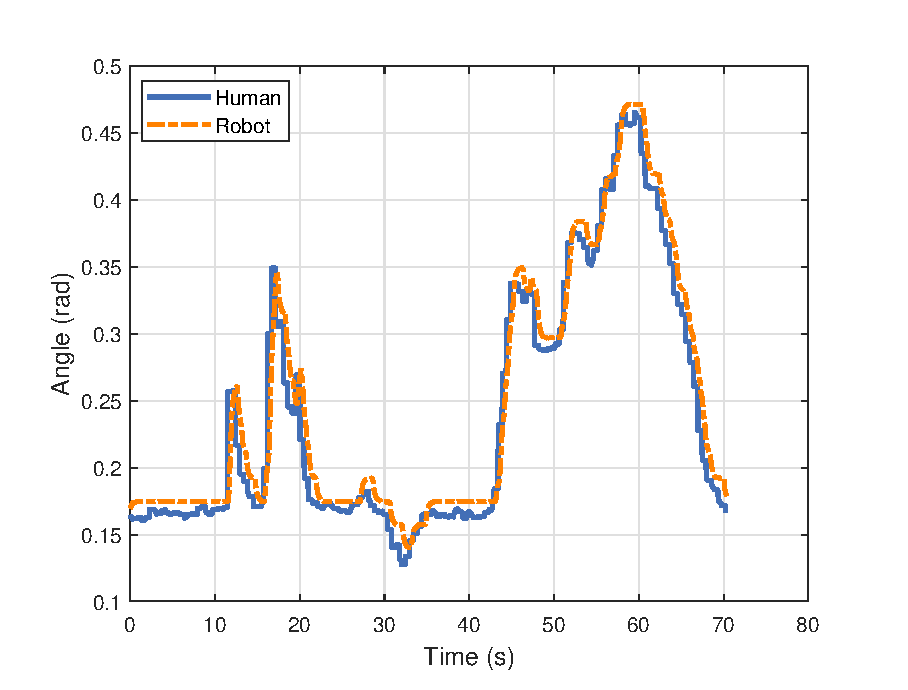
\includegraphics[width=0.44\linewidth]{Figure/chapter2/LSR.eps}%
	}\\[0.8em]  % ★ 在两排之间加一点竖直间距(可调)
	
	% 下排两幅图
	\subfloat[]{%
		\includegraphics[width=0.44\linewidth]{Figure/chapter2/LSY.eps}%
	}\hfill
	\subfloat[]{%
		\includegraphics[width=0.44\linewidth]{Figure/chapter2/LE.eps}%
	}
	
	\caption{上肢关节轨迹跟踪结果。(a) 肩关节屈伸;(b) 肩关节外展-内收;(c) 肩关节内外旋;(d) 肘关节屈伸。}
	\label{fig:upper_tracking}
\end{figure}


为进一步验证下肢部分的运动学跟踪性能,选取髋关节屈伸(Hip pitch)、髋关节外展(Hip roll)以及膝关节屈伸(Knee)作为代表性关节进行分析,图~\ref{fig:lower_tracking} 了左腿主要关节的轨迹跟踪结果。可以看出,机器人下肢关节轨迹整体能够保持与人体参考轨迹一致的变化趋势,曲线变化平滑,无明显震荡或异常跳变。相比上肢关节,下肢关节在运动过程中受骨盆结构与支撑约束影响较强,其角度变化呈现更为规律的趋势,因此通过几何关系推导得到的参考角具有较好的稳定性。这表明所提出的下肢几何建模方法在结构约束明确的条件下具有较好的鲁棒性。


\begin{figure}[H]
	\centering
	\begin{adjustwidth}{0cm}{0cm}
		\subfloat[]{\includegraphics[width=0.32\linewidth]{Figure/chapter2/Hip pitch.eps}}
		\hfill
		\subfloat[]{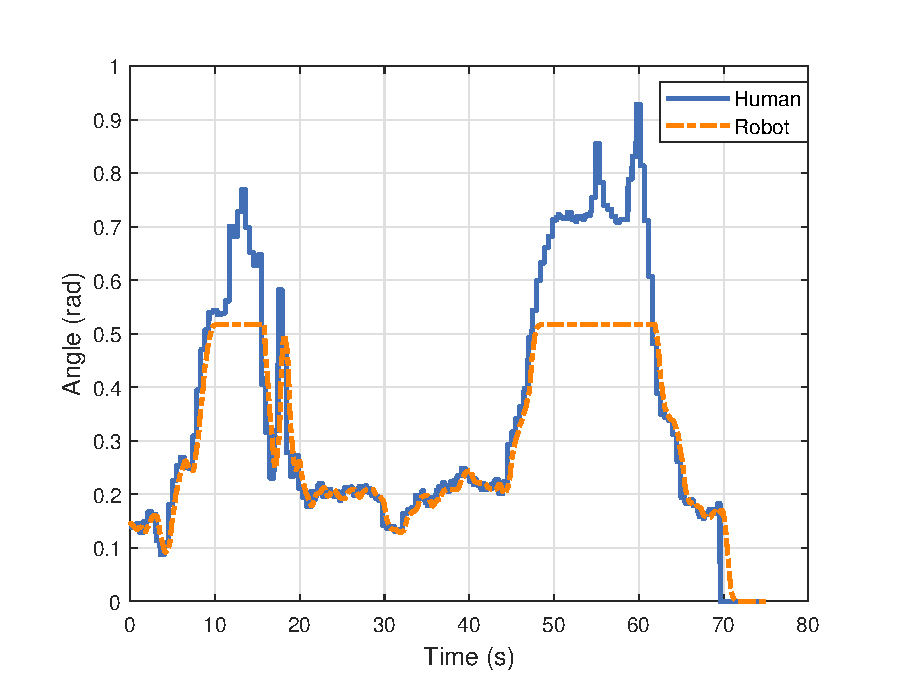
\includegraphics[width=0.32\linewidth]{Figure/chapter2/Hip_roll.eps}}
		\hfill
		\subfloat[]{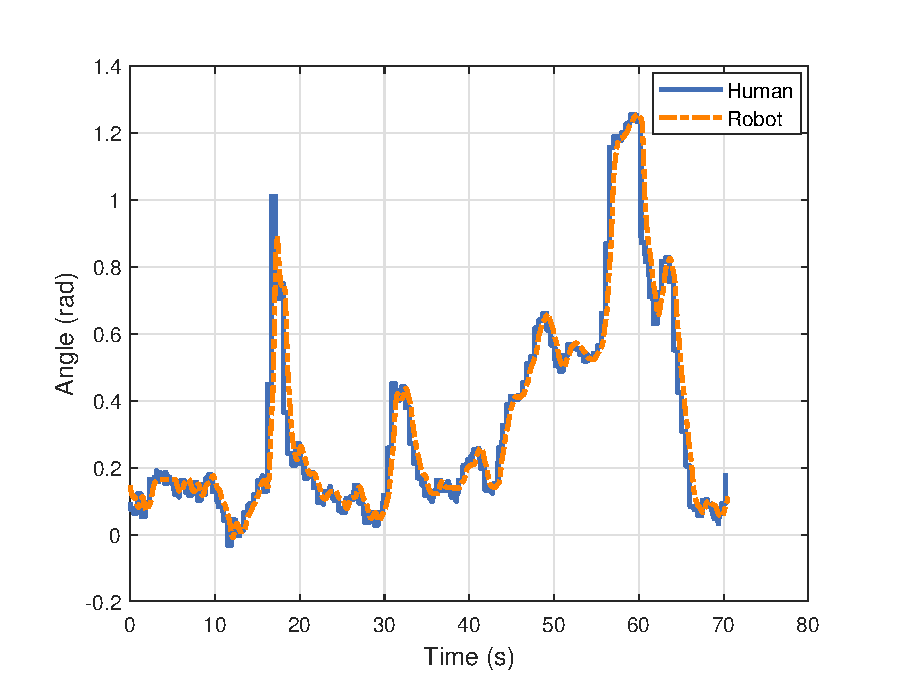
\includegraphics[width=0.32\linewidth]{Figure/chapter2/Knee.eps}}
	\end{adjustwidth}
	\caption{下肢关节轨迹跟踪结果:(a)髋关节屈伸;(b) 髋关节外展;(c) 膝关节屈伸。}
	\label{fig:lower_tracking}
\end{figure}



综合上肢与下肢的轨迹对比结果可以看出,全身运动学重定向方法能够在关节限位范围内实现较高精度的关节轨迹重构。尽管姿态估计噪声与执行器响应延迟会引入一定误差,但整体运动趋势保持一致,未出现明显的姿态畸变或构型失真现象,验证了该方法在全身层面的稳定性与一致性。


为进一步定量评估全身运动学重定向方法的跟踪精度,本文采用均方误差(Mean Square Error, MSE)作为关节轨迹误差评价指标,定义为 $\mathrm{MSE} = \frac{1}{T} \sum_{t=1}^{T} (q_{\mathrm{robot}}(t) - q_{\mathrm{ref}}(t))^2$,其中 $q_{\mathrm{robot}}(t)$ 为机器人实际关节角,$q_{\mathrm{ref}}(t)$ 为人体参考关节角。

图~\ref{fig:mse_all} 给出了各代表性关节的 MSE 统计结果。从图中可以看出,各关节误差整体处于较低水平,均小于 $0.11\,\mathrm{rad}^2$,表明所提出的全身重定向方法能够实现较高精度的运动学映射。

\begin{figure}[H]
	\centering
	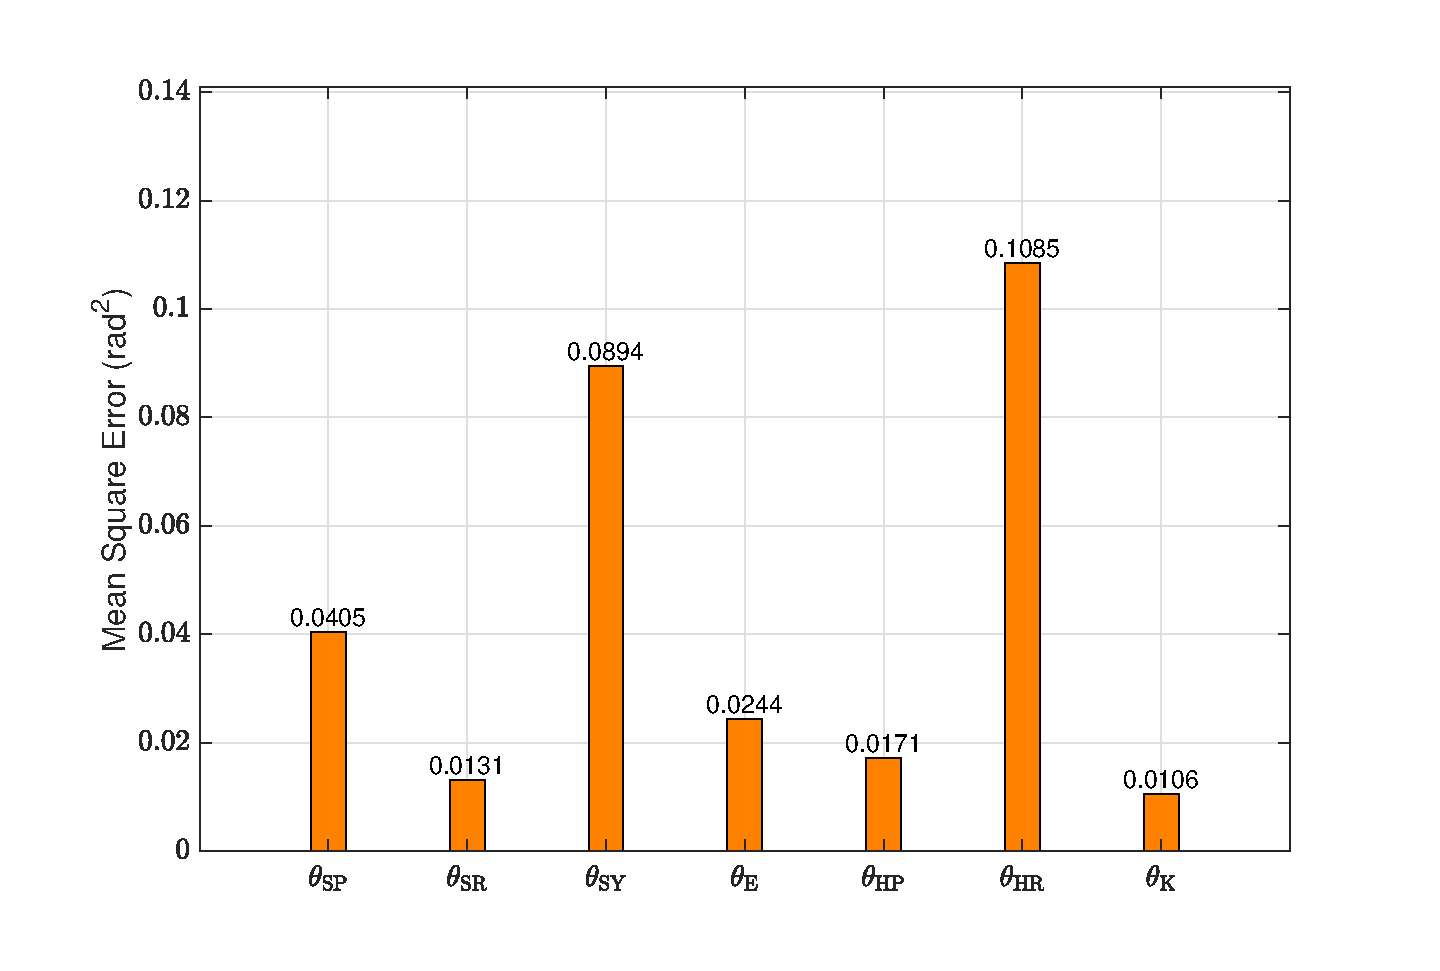
\includegraphics[width=0.8\textwidth]{Figure/chapter2/MSE.eps}
	\caption{全身关节均方误差(MSE)统计结果。}
	\label{fig:mse_all}
\end{figure}

从不同关节的误差分布来看,膝关节屈伸误差最小,肩关节外展-内收误差亦较小($0.0131\,\mathrm{rad}^2$),说明在几何约束明确且运动特征明显的关节上,重定向精度较高。髋关节屈伸误差为 ($0.0171\,\mathrm{rad}^2$),同样保持较低水平。相对而言,髋关节外展($0.1085\,\mathrm{rad}^2$)与肩关节内外旋($0.0894\,\mathrm{rad}^2$)的误差较大。这主要是由于这类关节对空间侧向位移与深度信息较为敏感,在姿态估计过程中容易受到关键点噪声影响,从而放大至关节角计算结果中。此外,机器人机械结构与人体自由度分布存在差异,也会对侧向旋转类关节产生一定影响。

总体来看,误差主要来源于姿态估计数据波动与执行器响应延迟,而非几何重定向模型本身的结构性缺陷。结合轨迹定性分析与误差定量统计结果可以得出,所提出的全身运动学重定向方法能够在保证关节构型合理性的前提下,实现较高精度的全身关节轨迹重构。

\subsection{全身末端位置误差分析}

除关节空间误差外,为进一步评估全身运动学重定向方法在任务空间层面的跟踪精度,本文对双手与双脚末端位置误差进行统计分析。

末端误差定义为机器人与人体在相对初始位姿下的位移增量误差。设 $t=0$ 时刻人体与机器人末端均位于原点位置,后续时刻末端位置相对于初始位置的增量作为运动目标,即
$
\mathbf{p}^{\Delta}(t) = \mathbf{p}(t) - \mathbf{p}(0).
$
则末端误差定义为
\begin{equation}
	e(t) = \left\| \mathbf{p}^{\Delta}_{\mathrm{robot}}(t) - 
	\mathbf{p}^{\Delta}_{\mathrm{human}}(t) \right\|.
\end{equation}

该定义能够消除初始对齐误差的影响,仅反映运动过程中的相对位移跟踪性能。例如,当人体手部沿 $x$ 方向移动 $5\,\mathrm{cm}$ 时,机器人末端亦需产生等幅度位移,误差由两者增量差值决定。

图~\ref{fig:end_eff_results}(a) 给出了四个末端在整个运动过程中的位置误差时间序列。可以观察到,所有末端误差在初始阶段由零逐渐增大,并在 $1\sim2\,\mathrm{s}$ 内进入稳定波动区间。整体误差维持在 $1\sim2.5\,\mathrm{cm}$ 范围内,未出现明显发散或持续累积现象,说明重定向过程中不存在系统性漂移。

\begin{figure}[H]
	\centering
	
	\begin{subfigure}{0.48\linewidth}
		\centering
		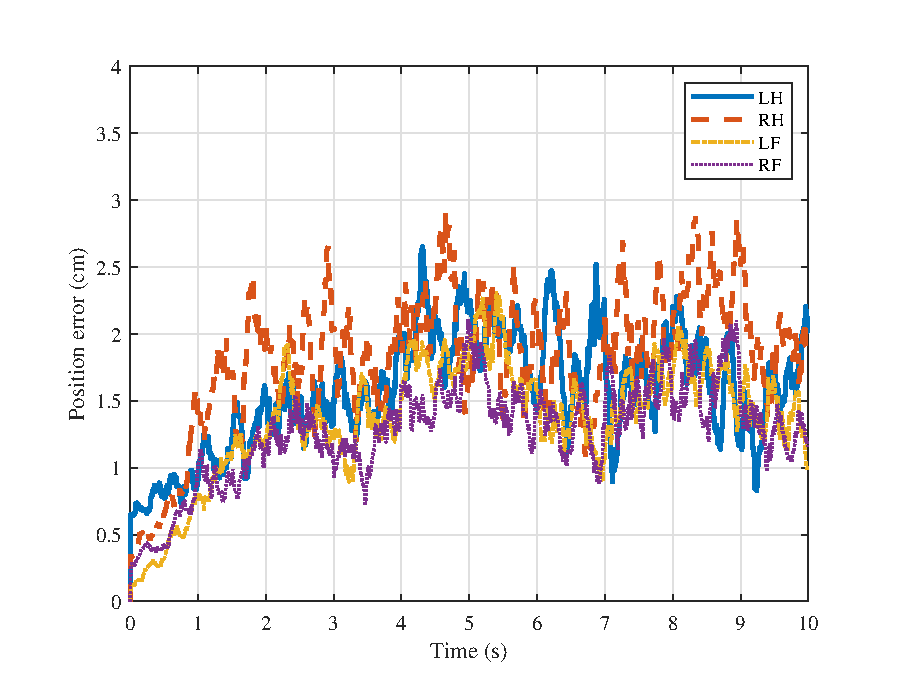
\includegraphics[width=\linewidth]{Figure/chapter2/end_xyz_err.eps}
		\label{fig:end_eff_time}
	\end{subfigure}
	\hfill
	\begin{subfigure}{0.48\linewidth}
		\centering
		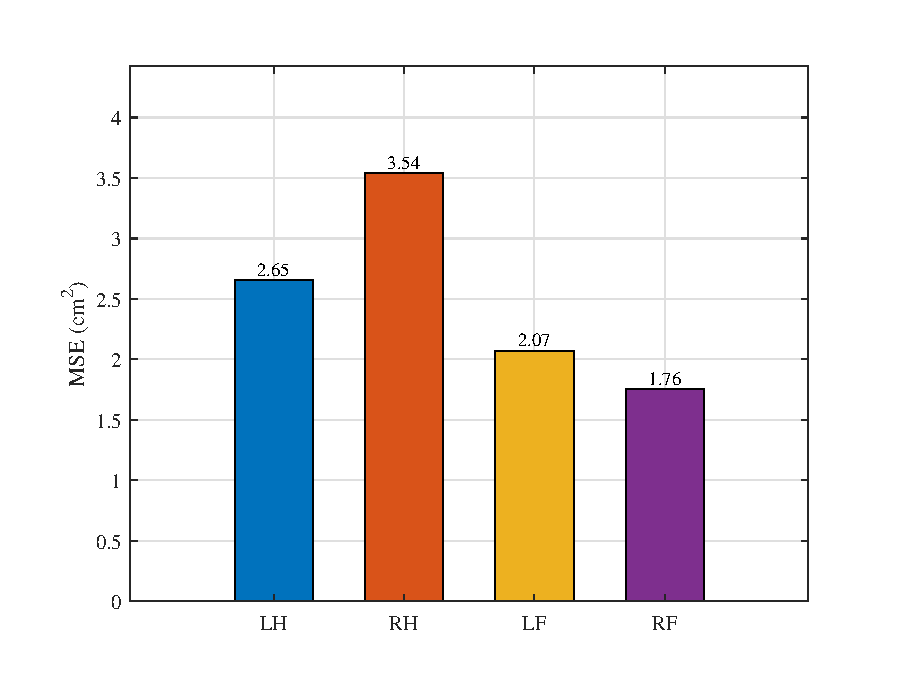
\includegraphics[width=\linewidth]{Figure/chapter2/end_MSE.eps}
		\label{fig:end_eff_mse}
	\end{subfigure}
	
	\caption{末端位置误差结果对比。
		(a) 双手与双脚末端位置误差时间序列;
		(b) 双手与双脚末端位置均方误差统计结果。}
	\label{fig:end_eff_results}
\end{figure}
从误差幅值对比来看,右手(RH)误差整体略高于左手(LH),峰值可达约 $2.5\,\mathrm{cm}$;双脚误差相对较低,左脚(LF)与右脚(RF)误差主要分布在 $1.0\sim1.8\,\mathrm{cm}$ 区间。这表明上肢末端在大幅度摆动阶段更易受到姿态估计噪声与运动幅度放大的影响,而下肢由于受骨盆结构与支撑约束限制,空间位移变化相对稳定。

为进一步定量评估误差水平,图~\ref{fig:end_eff_results}(b) 给出了各末端的均方误差(MSE)统计结果。从结果可见,右手误差最大($2.55\,\mathrm{cm}^2$),左手为 $2.10\,\mathrm{cm}^2$,左脚与右脚分别为 $1.58\,\mathrm{cm}^2$ 与 $1.60\,\mathrm{cm}^2$。整体误差均保持在较低水平,说明全身运动学重定向方法在任务空间层面能够实现较高精度的末端位置重构。


综合时间序列分析与统计结果可以看出,所提出的全身运动学重定向方法不仅能够在关节空间实现良好跟踪,同时在任务空间层面也能够保证末端位置的相对位移一致性。误差主要来源于姿态估计噪声以及执行器响应延迟,而非模型结构性缺陷。



\subsection{全身重定向消融实验}

为验证所提出全身运动学重定向方法在多末端约束与构型保持方面的有效性,本文设计消融实验,对以下方法进行对比:

1)纯几何映射方法(Geometry-based);  
2)解析逆运动学方法(IK);  
3)基于二次规划的优化方法(QP);  
4)本文提出的改进全身重定向方法。

对比指标包括:是否考虑关节限制、是否保持构型一致性、末端平均位置误差以及计算迭代次数。末端误差定义与前文一致,采用相对初始位姿的位移增量误差,并对双手与双脚四个末端取平均。统计结果如表~\ref{tab_ablation} 所示。

\begin{table}[ht]
	\centering
	\caption{不同全身重定向方法性能比较}
	\begin{tabular}{lcccc}
		\toprule
		方法 & 关节限制 & 构型约束 & 末端平均误差 (cm) & 迭代次数 \\
		\midrule
		几何方法 & $\times$ & \checkmark & 3.85 & $\times$ \\
		解析IK & $\times$ & $\times$ & 1.20 & 1 \\
		QP方法 & \checkmark & $\times$ & 1.85 & $\approx100$ \\
		改进重定向 & \checkmark & \checkmark & 1.52 & $\approx20$ \\
		\bottomrule
	\end{tabular}
	\label{tab_ablation}
\end{table}

从表~\ref{tab_ablation} 可以看出,纯几何方法由于未显式约束末端位置,导致全身末端平均误差最大。解析逆运动学方法能够精确满足末端位置约束,因此误差较小,但其未考虑关节限制与构型保持,容易产生不自然姿态或接近关节极限的解。

基于QP的优化方法在满足关节限制的同时实现了末端位置跟踪,误差明显优于几何方法,但由于缺乏构型保持项,冗余自由度下的姿态分布仍存在一定偏差,同时计算迭代次数较多。

本文提出的改进全身重定向方法在保证关节限制与构型约束的前提下,实现了较低的末端误差(1.52 cm),且仅需约20次迭代即可收敛,在精度与计算效率之间取得了更优平衡。



\subsubsection{主观评价实验}

为进一步评估全身动作模仿的自然性与可接受性,本文邀请六名参与者进行示范动作,由机器人执行对应重定向结果,并进行主观评分。评价指标包括:

1)动作平滑性(Motion Smoothness, MS);  
2)姿态可行性(Pose Feasibility, PF);  
3)任务完成度(Task Achievement, TA);  
4)总体用户偏好(Overall Preference, OP)。

评分采用 1(差)至 5(优)的五分制。统计结果如表~\ref{tab:user_evaluation} 所示。

实验结果表明,所提出的全身重定向方法在四项指标上均取得最高评分,尤其在姿态可行性与总体偏好方面优势明显。这说明在保证末端跟踪精度的同时,引入构型保持项能够显著提升动作自然性与用户接受度。



\begin{table}[htbp]
	\centering
	\caption{不同重定向方法的用户主观评价}
	\label{tab:user_evaluation}
	\begin{tabular}{lcccc}
		\toprule
		方法  & MS  & PF  & TA  & OP \\
		\midrule
		几何方法     & 4   & 5   & 2   & 4   \\
		逆运动学方法 & 4   & 2   & 3   & 2   \\
		QP 方法      & 3   & 3   & 3   & 3   \\
		本文方法     & 5   & 5   & 4   & 5   \\
		\bottomrule
	\end{tabular}
\end{table}

\section{结论与局限性讨论}
本文提出了一种面向全身运动学的改进重定向方法,在满足关节限位约束的前提下,通过引入构型保持项与多末端位置约束,实现了关节空间与任务空间的协同优化。该方法能够在保证末端位置跟踪精度的同时,维持合理的关节构型,从而提升动作的自然性与稳定性。

实验结果表明,在关节空间层面,机器人各主要关节能够较好地跟随人体参考轨迹变化趋势,未出现明显构型畸变或轨迹跳变现象;在任务空间层面,双手与双脚末端位置误差整体维持在厘米级范围内,且误差未出现随时间累积的漂移现象。消融实验进一步验证了构型保持项在全身重定向中的重要作用:相比纯几何映射与传统QP方法,所提出的方法在精度与计算效率之间取得了更优平衡。同时,通过引入多目标优化策略,该方法在实时性方面表现稳定,平均迭代次数显著低于传统QP求解框架,能够满足实时动作模仿的计算需求。

尽管本文方法在全身运动学重定向方面取得了良好效果,但仍存在一定局限性。首先,当前实验分析主要围绕末端位置跟踪与关节构型保持展开,对于完整姿态信息(包括位置与方向)的跟踪性能未进行单独量化讨论。事实上,所构建的QP优化框架本身可以通过引入姿态误差项对末端方向进行联合约束,但在本章实验中主要聚焦于位置约束与构型一致性,因此未对姿态方向误差进行系统统计分析。在涉及复杂旋转自由度(如前臂旋前-旋后或手腕复合运动)时,若未显式加入方向约束项,姿态重建精度可能受到一定影响。其次,本文研究重点集中于运动学层面的重定向问题,未显式引入动力学约束与接触稳定性条件。虽然在实验过程中未出现明显失稳或构型异常现象,但在高动态动作或复杂接触环境下,单纯基于运动学优化可能不足以保证系统稳定性。未来可结合层级QP或全身动力学控制框架,将运动学重定向结果进一步映射至力控制层,从而提升系统在复杂任务中的稳定性与鲁棒性。此外,姿态估计噪声与执行器响应延迟仍然是影响重定向精度的主要因素。尽管当前系统误差保持在厘米级与较低关节误差范围内,但在更高精度或高速动作场景中,关键点波动与控制滞后可能进一步放大误差。

未来工作将从两个方面展开:一是将运动学重定向结果与全身动力学控制方法相结合,提升复杂场景下的稳定性与可控性;二是结合学习型方法增强系统对未见动作与复杂任务的泛化能力,从而进一步拓展全身动作模仿的应用范围。